As máquinas assíncronas são as mais utilizadas pela industria. Nessas máquinas, tanto o rotor quanto o estator operam em corrente alternada. A corrente que circula pelo rotor é uma corrente induzida por um campo magnético variável em relação ao enrolamento do rotor. Esse campo magnético é variável devido à diferença de velocidade entre o rotor e o campo magnético girante. Por isso são chamadas costumeiramente de máquinas de indução. As máquinas de indução podem ser utilizadas como motores e como geradores.

\begin{figure}[ht]
    \center
    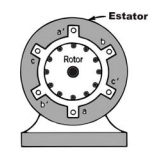
\includegraphics[scale=1]{imagens/8}
    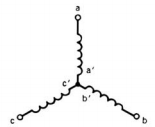
\includegraphics[scale=1]{imagens/9}
    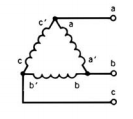
\includegraphics[scale=1]{imagens/10}
    \caption{Representação da máquina Assíncrona}
\end{figure}

